%% The comment character in TeX / LaTeX is the percent character.
%% The following chunk is called the header

\documentclass{article} % essential first line
\usepackage{times}    % this uses fonts which will look nice in PDF format
\usepackage{graphicx}   % needed for the figures
\usepackage{url}
\usepackage{adjustbox}
\usepackage{amsmath}
\usepackage{listings}
\usepackage{color}

\definecolor{dkgreen}{rgb}{0,0.6,0}
\definecolor{gray}{rgb}{0.5,0.5,0.5}
\definecolor{mauve}{rgb}{0.58,0,0.82}

\lstset{frame=tb,
  language=Java,
  aboveskip=3mm,
  belowskip=3mm,
  showstringspaces=false,
  columns=flexible,
  basicstyle={\small\ttfamily},
  numbers=none,
  numberstyle=\tiny\color{gray},
  keywordstyle=\color{blue},
  commentstyle=\color{dkgreen},
  stringstyle=\color{mauve},
  breaklines=true,
  breakatwhitespace=true,
  tabsize=3
}

%% Set the folder where pictures are located
\graphicspath{ {figures/} }

%% Here I adjust the margins

\oddsidemargin -0.25in    % Left margin is 1in + this value
\textwidth 6.75in   % Right margin is not set explicitly
\topmargin 0in      % Top margin is 1in + this value
\textheight 9in     % Bottom margin is not set explicitly
\columnsep 0.25in   % separation between columns

%% Define a macro for inserting postscript images
%% ==============================================
%% This is a macro which nominally takes 3 parameters, 
%% it would be used as follows to insert and encapsulated postscript
%% image at the location where it is used.
%%
%% \EPSFIG{epsfilename}{caption}{label}
%% - epsfilename is the name of the encapsulated postscript file to be
%%               inserted at this location
%% - caption is the text to be shown as the figure caption, it will be
%%           prepended by Figure X.  The number X can be referenced
%%           using the label parameter.
%% - label is a name given to the figure, it can be referenced using the
%%         \ref{label} command.

%\def\EPSFIG[#1]#2#3#4{   % Don't be scared by this monsrosity
%\begin{figure}[hbt]    % it is a macro to save typing later
%\begin{center}     % 
%\includegraphics[#1]{#2} %
%\end{center}     %
%\caption{#3}     %
%\label{#4}     %
%\end{figure}     %
%}        %

%% Define the fields to be displayed by a \maketitle command
\author{Timothy Dee, Brent Barth}
%{\it Undergraduate, Department of Electrical and Computer Engineering, Iowa State University}
%\author{Brent Barth}
%\it Undergraduate, Department of Electrical and Computer Engineering, Iowa State University}
\title{GUI Car Simulation with Processor Depiction}

%%
%% Header now finished
%%

\begin{document}    % Critical
\twocolumn
\thispagestyle{empty}   % Inhibit the page number on this page
\maketitle      % Use the \author, \title and \date info

%% Next comes the abstract, notice the curly-braces surrounding the
%% text.

%%%%%%%%%%%%%%%%%%%%%
% PROJECT DESCRIPTION
%%%%%%%%%%%%%%%%%%%%%
%		CprE 458/558 Term Project Report Format (Sample)
%==========================================================================
%
%Here are some guidelines for the report. Page limits are mere suggestion,
%use number of pages as appropriate.
%
%There are three types of reports - survey, simulation, and implementation.
%
%Simulation/Implemenation Report Format (12-15 pages):
%
%       Project Summary  (1 page)
%       1. Introduction (2 pages)
%       2. Objectives and Scope (1 page)
%          Problem statement and Assumptions.
%       3. Solution Approach (3-4 pages)
%          3.1. Algorithm/Protocol (Discussion about the algo/protocol).
%          3.2 Illustrative Example
%       4. Simulation/Implementation (5 pages)
%          4.1. Simulation Model / Experimental Environment
%          4.2  Experiments and Analysis / Implementaion Details
%          4.3  Performance plots/ sample outputs / Sample screen output for GUI based simulator
%       5. Conclusions (3 pages)
%          5.1. Conclusion of the report; also, identify future work if relevant).
%          5.2  What did you learn by this project
%          5.3  Suggestion for such projects (feedback to the instructor)
%       References 
%%%%%%%%%%%%%%%%%%%%%%%%%%%%%%%%%%%%%%%%%%%%%%%%%%%%%%%%%%%%%%%%
% report should convey some sort of learning, beyond what we learned in class

\abstract{This report describes a gui simulation created for Cpre 458, Real Time Systems. 
The simulation depicts a car driving and the state of the processor on the car. 
The car is shown to be reacting to obstacles in accordance to the tasks being submitting.
The tasks are represented visually in a panel which depicts the state of the processor.
This paper also discusses the specific implementation of the program.
This project design was inspired by the idea of autonomous driving, similar to Google Car.}

% Insert description from original project proposal
\section{Project Summary}
The goal of this project is to learn about the challenges associated with implementing a real-time system.
In accordance with this goal, it is necessary to think about real-life situation which can be modeled by simple means.
For purposes of this project, the situation must be scalable so a basic working version may be reached relatively swiftly while working toward the more complex desirable implementation.
For this reason, we choose to implement a simple version of an autonomous driving system.

The reason such a problem is a good candidate is due several factors.
First, the rules are well defined. Most people can easily understand what a car should do when it is on the road. This makes our depiction of the car easy to understand.
Second, such a problem is also scalable because an arbitrary number of objects which require some nature of response may be introduced.

The implementation of this system will need to visually represent a car driving on a road.
There will also need to be clear obstacles presented to the car.
Internally our program will need to use the ideas presented in Real-Time Systems to cause the car to react to the obstacles.
This internal state will also need to be visually depicted.
%TODO

\section{Introduction}
%TODO

\section{Objectives and Scope}
%TODO

\section{Solution Approach}
\subsection{Algorithms}
%TODO

% give an example of our thing running i suppose?
\subsection{Solution Sample}
%TODO

\section{Simulation}
We seek to implement a system which demonstrates how the ideas from Real Time Systems may be applied to the autonomous driving problem.
For this, we choose to implement three distinct logical components.
First, we create an entity which keeps track of the state of the \'world\'. This entity will need to show this \'world\' based on the current state, and update the state. It will also need to derive information from the current state of the \'world\' which will enable the processing entity to know if it needs to cause the car to react to an obstacle.
Second, there must exist a sort of processing unit which maintains a list of tasks and performs the scheduling. This processing unit takes information from the first entity which maintains the state of the \'world\', using this information to modify on what element  processing will be done.
Third, There is a unit which takes in information regarding the state of the processing and shows it visually.

% block diagram of classes should probabally go here
\subsection{Simulation Model}
% Diagram of code
\begin{figure}[!hbt]
\begin{center}
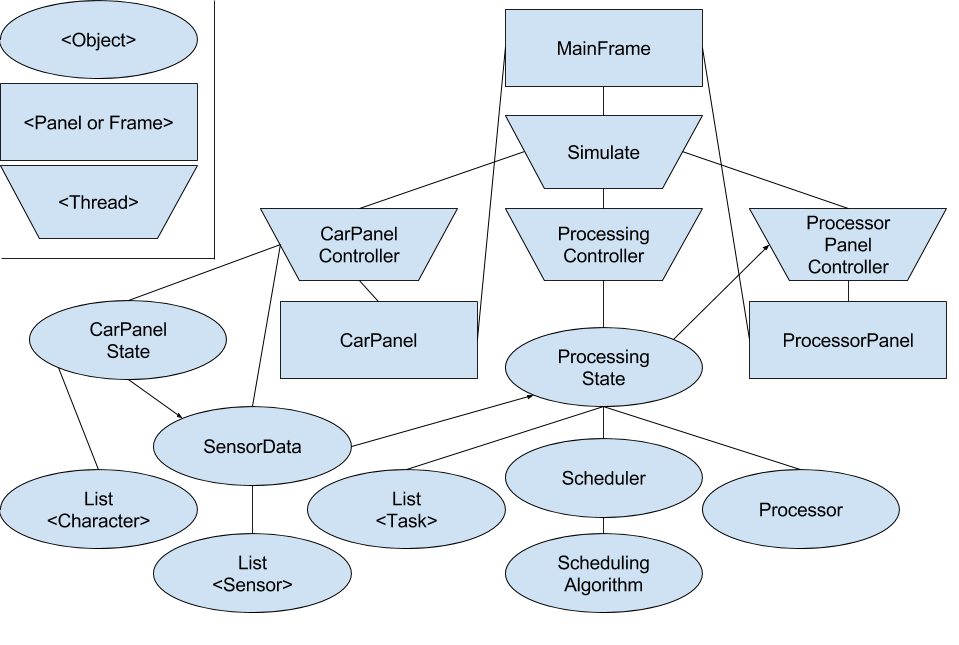
\includegraphics[width=.4\textwidth,keepaspectratio]{code_layout.png}
\end{center}
\caption{Program Layout}
\label{FIG-DIAGRAM}
\end{figure}

Our program code follows a structure having objects with purpose similar to the logical components discussed in the preface of this section.
Figure \ref{FIG-DIAGRAM} illustrates this layout.
In this diagram, lines drawn between two entities represent a control relationship. The MainFrame, for example, controls the Simulate thread.
The Simulate thread, in turn, controls three additional threads. Each of these threads is preforming tasks consistent with the logical component they represent.
Arrows represent the flow of information.

In the diagram it can be seen that information flows from CarPanelState to SensorData to ProcessingState and finally to ProcessorPanelController.
Each of these objects or threads consume the information produced by the previous.object or thread.
CarPanelState is updated by CarPanelController using logic which is consistent with the laws of physics.
This means if an object has a nonzero speed than it will move in accordance with that speed on each update of the panel.
%TODO

% present code and explanations for design choices here
\subsection{Implementation Details}
Discussed here are the specific implementation details and program design choices.
The overall design philosophy utilized delegates as much processing as possible until it becomes trivial..
This means that components higher in the hierarchy should not need to have any knowledge of how the lower components preform their function.
A specific example of this is objects which represent a graphical element knowing how to draw themselves. In this example, the panel which contains the graphical element would ask it to draw itself, this is the delegation of work. 

% in each subsubsection, state:
% what the class is used to accomplish
% how the class fits into the overall program design
% important design decisions made in that class
% how this class interacts with other classes
\subsubsection{MainFrame}
% code used to set up the threads
\begin{lstlisting}[caption={Setup Threads},label={lst:threads},numbers=left]
// add the panels to this frame
CarPanel car_panel = new CarPanel(this.width, this.height);
ProcessorPanel processor_panel = new ProcessorPanel();
this.add(car_panel);
this.add(processor_panel);

// start any necessary threads
CarPanelController car_controller = new CarPanelController(car_panel);
ProcessorPanelController processor_controller = new ProcessorPanelController(processor_panel);
ProcessingController processing_controller = new ProcessingController(scheduling_algorithm, n_processors);

Thread car_controller_thread = new Thread(car_controller);
Thread processor_controller_thread = new Thread(processor_controller);
Thread processing_controller_thread = new Thread(processing_controller);
    
// start these threads, but they don't act autonamously. Simulate thread
// will use them to perform the simulation.
car_controller_thread.start();
processor_controller_thread.start();
processing_controller_thread.start();

// START SIMULATION THREAD
Simulate simulator = new Simulate(car_controller, processor_controller, processing_controller, width, height);
Thread simulator_thread = new Thread(simulator);
simulator_thread.start();
\end{lstlisting}

This class is used to establish properties of the main window for program simulation.
The goal of this class is to arrange the different visual components of the program and begin the simulation.
Here is where necessary design decisions about how the responsibilities of the program are delegated.
The choice was made to divide the responsibility among three different threads. An addition thread is used to coordinate activity between these threads.
Listing \ref{lst:threads} shows the initialization of threads and how they are given to the fourth thread to be managed.

\subsubsection{Simulate}
% shows the update procedure in the simulate thread
\begin{lstlisting}[caption={Simulate Update Procedure},label={lst:simulate},numbers=left]
while (true) {
  try {
    // update every 3ms
    Thread.sleep(3);
  } catch (Exception e) {
    e.printStackTrace();
  }

  // provide the SensorData to the ProcessingController
  this.processing_controller.set_sensor_data(this.car_panel_controller.get_sensor_data());

  // provide the processing state to the processor panel
  this.processor_panel_controller.set_processing_state(this.processing_controller.get_state());
}
\end{lstlisting}


This thread has two goals. It's primary purpose is to coordinate activity between the threads which manage the visual components and the processing.
This thread's secondary goal is to set up all of the obstacles and periodic tasks used in the simulation.
\ref{lst:simulate}
%TODO

\subsubsection{CarPanelController}
\begin{lstlisting}[caption={Panel Update Procedure},label={lst:carpanelcontroller},numbers=left]
private void update_panel() {
  // update the targets if necessary
  update_target_state();

  // call methods to perform various specific updates
  move_car();
  move_obstacles();
  move_other_cars();
  move_signs();
  move_road();

  // cause the panel and its children to repaint
  this.car_panel.repaint();
  this.car_panel.revalidate();
}
\end{lstlisting}

\ref{lst:carpanelcontroller}
%TODO

\subsubsection{ProcessingController}
\begin{lstlisting}[caption={Processing Controller Update Procedure},label={lst:ProcessingController},numbers=left]
while (true) {
  try {
    // update every 10 ms (100 fps)
    Thread.sleep(10);
  } catch (Exception e) {
    e.printStackTrace();
  }

  // ask the state to update itself
  processing_state.update(1L);
}
\end{lstlisting}

\ref{lst:ProcessingController} depicts the update process for processing controller
%TODO

\subsubsection{ProcessorPanelController}
\begin{lstlisting}[caption={},label={lst:ProcessingPanelController},numbers=left]
while (true) {
  try {
    // update every 10 ms (100 fps)
    Thread.sleep(10);
  } catch (Exception e) {
    e.printStackTrace();
  }

  set_processing_state(this.processor_panel.getState());
  
  // cause the processor panel to be repainted
  processor_panel.repaint();
  processor_panel.revalidate();
}
\end{lstlisting}

\ref{lst:ProcessingPanelController}
%TODO

\subsubsection{CarPanel}
\begin{lstlisting}[caption={Ask Signs to Draw Themselves},label={lst:CarPanel},numbers=left]
for (Sign c : state.signs) {
  c.draw(g);
}
\end{lstlisting}

\ref{lst:CarPanel} illustrates the design philosophy. 
This shows how components are asked to draw themselves.
%TODO

\subsubsection{CarPanelState}
\begin{lstlisting}[caption={},label={lst:CarPanelState},numbers=left]
public MainCar main_car;
public Road road;

public ArrayList<Cone> obstacles;
public ArrayList<Car> other_cars;
public ArrayList<Sign> signs;
\end{lstlisting}

\ref{lst:CarPanelState}
%TODO

\subsubsection{Character}
\begin{lstlisting}[caption={},label={lst:character},numbers=left]
public void draw(Graphics g) {
  // draw the body of the car
  g.setColor(this.color);
  g.fillRect(this.x_pos, this.y_pos, this.width, this.height);

  if (Facing.RIGHT == this.facing) {
    // draw the windshield
    g.setColor(Color.black);
    g.fillRect(this.x_pos + this.width / 2 + this.width / 16, this.y_pos + this.height / 10, this.width / 3,
        this.height * 4 / 5);
  } else {
    // draw the windshield
    g.setColor(Color.black);
    g.fillRect(this.x_pos + this.width / 16, this.y_pos + this.height / 10, this.width / 3,
        this.height * 4 / 5);
  }
}
\end{lstlisting}

\ref{lst:character}
%TODO

\subsubsection{SensorData}
\begin{lstlisting}[caption={},label={lst:SensorData},numbers=left]
public StopSignSensor stop_sign_sensor;
public SpeedSignSensor speed_sign_sensor;
public OtherCarSensor other_car_sensor;
public ConeSensor cone_sensor;
\end{lstlisting}

\ref{lst:SensorData}
%TODO

\subsubsection{Sensor}
\begin{lstlisting}[caption={Implementation of Sensor},label={lst:sensor},numbers=left]
public class StopSignSensor extends Sensor {
  public ArrayList<Sign> signs;
  public ArrayList<Double> distances;

  public StopSignSensor(CarPanelState state) {
    super(state);
  }

  @Override
  protected void compute() {
    this.signs = new ArrayList<Sign>();
    this.distances = new ArrayList<Double>();

    for (Sign sign : this.car_panel_state.signs) {
      if (sign.type == SignType.STOP && is_within_range(this.car_panel_state.main_car, sign)) {
        // if within range of sensor
        signs.add(sign);

        // add in parallel the distance to the sign
        distances.add(compute_distance(this.car_panel_state.main_car, sign));
      }
    }
  }
}
\end{lstlisting}

\ref{lst:sensor}
%TODO

\subsubsection{ProcessingState}
\begin{lstlisting}[caption={},label={lst:ProcessingState},numbers=left]
private void update_processors(long time) {
  // preform updates in an incremental fashion
  for (int i = 0; i < time; i++) {
    // if a task has completed, run the scheduler at the point it
    // completes.
    // remember the only tasks who's computation time is decreasing are
    // the ones in the processors.
    for (Processor p : processors) {
      // first, decrement the computation time of the thing in this
      // processor
      p.task.computation_time_remaining--;

      if (p.task.computation_time_remaining <= 0) {
        // periodic tasks need to be added back
        if (p.task.nature == Task.Nature.PERIODIC) {
          // add the same task back in if it is periodic
          this.scheduler_task_queue.add(new Task(p.task.computation_time_origional, p.task.period,
              p.task.deadline, p.task.nature, p.task.action, p.task.processing_controller,
              p.task.car_panel_controller, p.task.set_point));
        }

        // preform the complete action of the task when it is
        // finished
        p.task.preform_action();

        // if the task has finished, get the next thing out of the
        // queue
        // set the current processor task to the smallest thing in
        // the queue
        if (p.task_queue.isEmpty() == false) {
          // get the next task in the queuue
          p.task = p.task_queue.get(0);

          // remove this task from the queue
          p.task_queue.remove(0);
        } else {
          // insert a dummy task
          p.task = new Task(1, 0, 0, Nature.APERIODIC, Action.NONE, null, null, 0);
        }
      }
    }
  }
}
\end{lstlisting}

\ref{lst:ProcessingState}
%TODO

\subsubsection{Task}
\begin{lstlisting}[caption={},label={lst:task},numbers=left]
// says what action should be conducted upon task completion
public enum Action {
  NONE, SET_CAR_SPEED, MOVE_UP_CAR, MOVE_DOWN_CAR, READ_CONE_SENSOR, READ_OTHER_CAR_SENSOR, READ_SPEED_SIGN_SENSOR, READ_STOP_SIGN_SENSOR;
}

public void preform_action()
\end{lstlisting}

\ref{lst:task}
%TODO

\subsubsection{Scheduler}
\begin{lstlisting}[caption={},label={lst:scheduler},numbers=left]
/**
 * returns the task set in scheduled order. null if not schedulable.
 */
public ArrayList<List<Task>> schedule(List<Task> tasks, int n_processors) {
  ArrayList<Task> array_list_tasks = new ArrayList<Task>(tasks);

  return this.scheduling_algorithm.schedule(
    array_list_tasks, n_processors);
}
\end{lstlisting}

\ref{lst:scheduler}
%TODO

\subsubsection{SchedulingAlgorithm}
\begin{lstlisting}[caption={},label={lst:SchedulingAlgorithm},numbers=left]
public interface SchedulingAlgorithm {
  /**
   * returns a schedule of all tasks for n processors. Each processor has a
   * different list in the task set.
   * 
   * @param tasks
   * @return
   */
  public List<List<Task>> schedule(List<Task> tasks, int n_processors);
}
\end{lstlisting}

\ref{lst:SchedulingAlgorithm}
%TODO

\subsubsection{Processor}
\begin{lstlisting}[caption={},label={lst:processor},numbers=left]
public Task task;
public List<Task> task_queue;
\end{lstlisting}

\ref{lst:processor}
%TODO

\subsubsection{ProcessorPanel}
\begin{lstlisting}[caption={},label={lst:ProcessorPanel},numbers=left]
protected void paintComponent(Graphics g) {
  super.paintComponent(g);

  drawSchedulerQueueTasks(g);
  drawTaskTables(g);
  drawLabels(g);
  draw_signs(g);
}
\end{lstlisting}

\ref{lst:ProcessorPanel}
%TODO

% put a picture of the GUI screen here
\subsection{Outputs}
%TODO

\section{Conclusion}
% what was good, what was bad
% what went well, what did not go well
\subsection{Synopsis}
%TODO

\subsection{Learning}
%TODO

\subsection{Suggestions}
It is good that the project is open-ended.
This gave us an opportunity to learn in a way which is interesting to us.
I felt a lot more motivated to do this project then I would have if it was a normal well-defined, highly-structured project.
It is much nicer to learn this way in my opinion.

I think it would be better if the project began earlier in the semester.
Having the start of the project be less than three weeks before dead week put a huge strain on time at this point in the semester.
I understand that it doesn't make sense to start the project before a significant amount of material has been covered.
Potentially making the report requirement slightly less substantial would help.
%TODO


% listing example
%\begin{lstlisting}[float=*,caption={Dynamic Frequency Scaling Mode II},label={lst:DFS_2},numbers=left]
%hi
%\end{lstlisting}

%% This bit generates the references.  This part starts to get
%% slightly tricky.
\bibliographystyle{unsrt} % Order by citation
\bibliography{report}

\end{document}
